\documentclass[11pt,a5paper,twoside]{article}
\usepackage{csjmol}

\usepackage{amssymb}
\usepackage{amsmath,amsthm,amsfonts}

\usepackage{graphicx}
\usepackage{doi}
%%% or you can use for figures the package
%%% \usepackage{epsfig}

\usepackage[usenames]{color}

\StartPage{1}

\CopyRight{2024 by Computer Science Journal of Moldova \\ \doi{10.xxxxxxxxxxx}}


\Headings{FN1. LastName1, FN2. LastName2, FN3. LastName3}
         {Short title of the paper \ldots}

\tolerance 1000

\title{The title of the paper}

\author{FirstName1 LastName1, FirstName2 LastName2, \and FirstName3 LastName3}
%\author{William Shakespeare, Ernest Hemingway, \and Abraham Lincoln}

\renewcommand{\CaptionChar}{. }


\newtheorem{definition}{Definition}
\newtheorem{theorem}{Theorem}
\newtheorem{lemma}{Lemma}
\newtheorem{algorithm}{Algorithm}
\newtheorem{example}{Example}


\newcommand{\V}{\mathcal{V}}
\newcommand{\lc}{\mathrm{lc}}
\newcommand{\mdeg}{\mathrm{mdeg}}


\begin{document}
\maketitle

\begin{abstract}
Place here short abstract in English. Please, do not exceed 
100 words.
\footnote{\ \ This work was supported by YYYYYYY project Ref. Nr. XXXXXXXXX} 
\footnote{\ \ To prepare the text for this template, parts of the texts from articles published in previous issues of CSJM were taken.}
The Computer Science Journal of Moldova (CSJM) publishes original articles and short communications which describe new scientific results in the domain closely related to Computer Science.

\textbf{Keywords:} Place here the words and phrases that better describe the content of your article, for example, computer science, information technologies (do not exceed 5-6 terms).

\textbf{MSC 2020:} Place here several codes of items from Mathematics Subject Classification 2020, for example, 68R10, 68Q25, 05C35, 05C05 mapping the subject of your article.
\end{abstract}

\section{Introduction}\label{sect1}
The authors for Computer Science Journal of Moldova (CSJM) are requested to follow instructions given in this sample paper. This template provides authors with most of needed formatting specifications.

The CSJM Editorial Board recommends preparing paper using this template style set. The paper should be 4--25 pages long. The format of the page is A5.

Articles should be submitted only in English. The authors are fully responsible for the content, presentation, and global typesetting aspects of the text, figures, tables (and all the attached materials).

One of the main requirements of the CSJM Editorial Board for the article design is a good level of English. Please, read your article once more before submitting it to the editorial board. Perhaps, you need the advice of some native speaker or a proofreader. Articles with a low level of English complicate even the review process, not to mention the reading and understanding of the text by readers of the article.


\section{Title of section 2}\label{sect2}
To prepare your articles for CSJM, please, use style csjmol.sty and the file CSJM\_template.tex as the template. The page margins, size, line spaces, and text fonts are prescribed in this style. If some specific styles are used for your article layout, please give the respective .sty files together with the main .tex file containing the text of your article. 

Please make sure that your additional styles and packages do not distort the CSJM format.

\section{Title of section 3}\label{sect3}
At the beginning of the article, provide the article title and the list of authors. The authors' names and surnames should be written using Western name order: first name or its initials should be written before the last name (surname). Then abstract, keywords, and MSC 2020 codes should be given. 
Abstract should be about 100 words. 

At the end of the article, the author’s affiliation (institution, address, E-mail, ORCID) must be indicated.

Article text may be divided in a number of sections, subsections, and subsubsections. 

Equations should be centered and labelled. Equation numbers, within 
parentheses, are to be positioned flush right, as in Eq. (\ref{eq1}).

\medskip
\noindent Example of equation Eq. (\ref{eq1}):
\begin{equation}
\label{eq1}
\frac{\partial ^2i}{\partial x^2}=\frac{LC}{\left( {\Delta {\kern 1pt}x} 
	\right)^2}\frac{\partial ^2i}{\partial t^2}+\frac{L}{\left( {\Delta {\kern 
			1pt}x} \right)^2R}\frac{\partial i}{\partial t}.
\end{equation}

Larger equation must be split in multiple lines, as in Eq. (\ref{eq2}). Number equations consecutively.

\medskip
\noindent Example of equation Eq. (\ref{eq2}):
\[
S(x)=f_i +(f_{i+1} -f_i )t+\frac{h_i^2 M_i (1-t)((1-t)^{\alpha _i 
	}-1)}{\alpha _i (\alpha _i +1)}+
\]
\begin{equation}
\label{eq2}
+\frac{h_i^2 M_{i+1} t(t^{\alpha _i }-1)}{\alpha _i (\alpha _i +1)},
\end{equation}
\textit{where the following notations are used:}
\[
t=(x-x_i )/h_i ,h_i =x_{i+1} -x_i ,S"(x_i )=M_i .
\]

\subsection{Example of subsection 1}
All figures must be stored in *.eps, 
.png, .pdf, or .jpg formats with a minimum 
resolution of 300 dpi. Be sure that your figures are of high quality. Each figure must have a caption under the figure (see Fig. \ref{fig1}).

\begin{figure}[htbp]
	\centerline{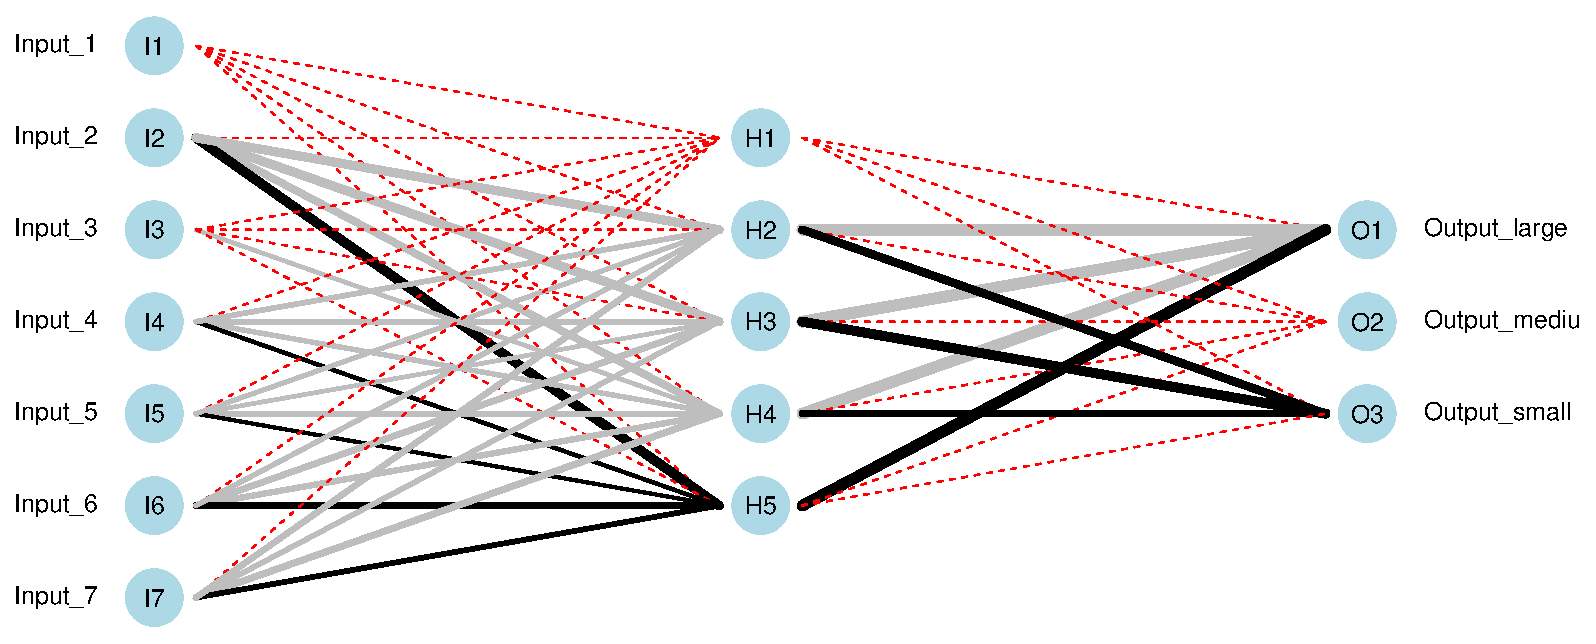
\includegraphics[width=10cm,height=5cm]{fig1.eps}}
	\caption{Caption for Figure 1}\label{fig1}
\end{figure}

\subsection{Example of subsection 2}
When you refer to an equation, a figure, a table, a section, or literature references in the text of the paper, please, use the following expressing: Eq. (\ref{eq1}), Eqs. (\ref{eq1}) and (\ref{eq2}), (see Fig.\ref{fig2}), Table \ref{tab1}, Section \ref{sect1}, \cite{1}, \cite{1} --\cite{3}. The use of direct notation, such as Eq. (1), Eqs. (1) and (2), (see Fig. 2), Table 1, Section 1, [1], [1-3], is also acceptable.

\begin{figure}[htbp]
	% Use the relevant command to insert your figure file.
	% For example, with the graphicx package use
	\centering
	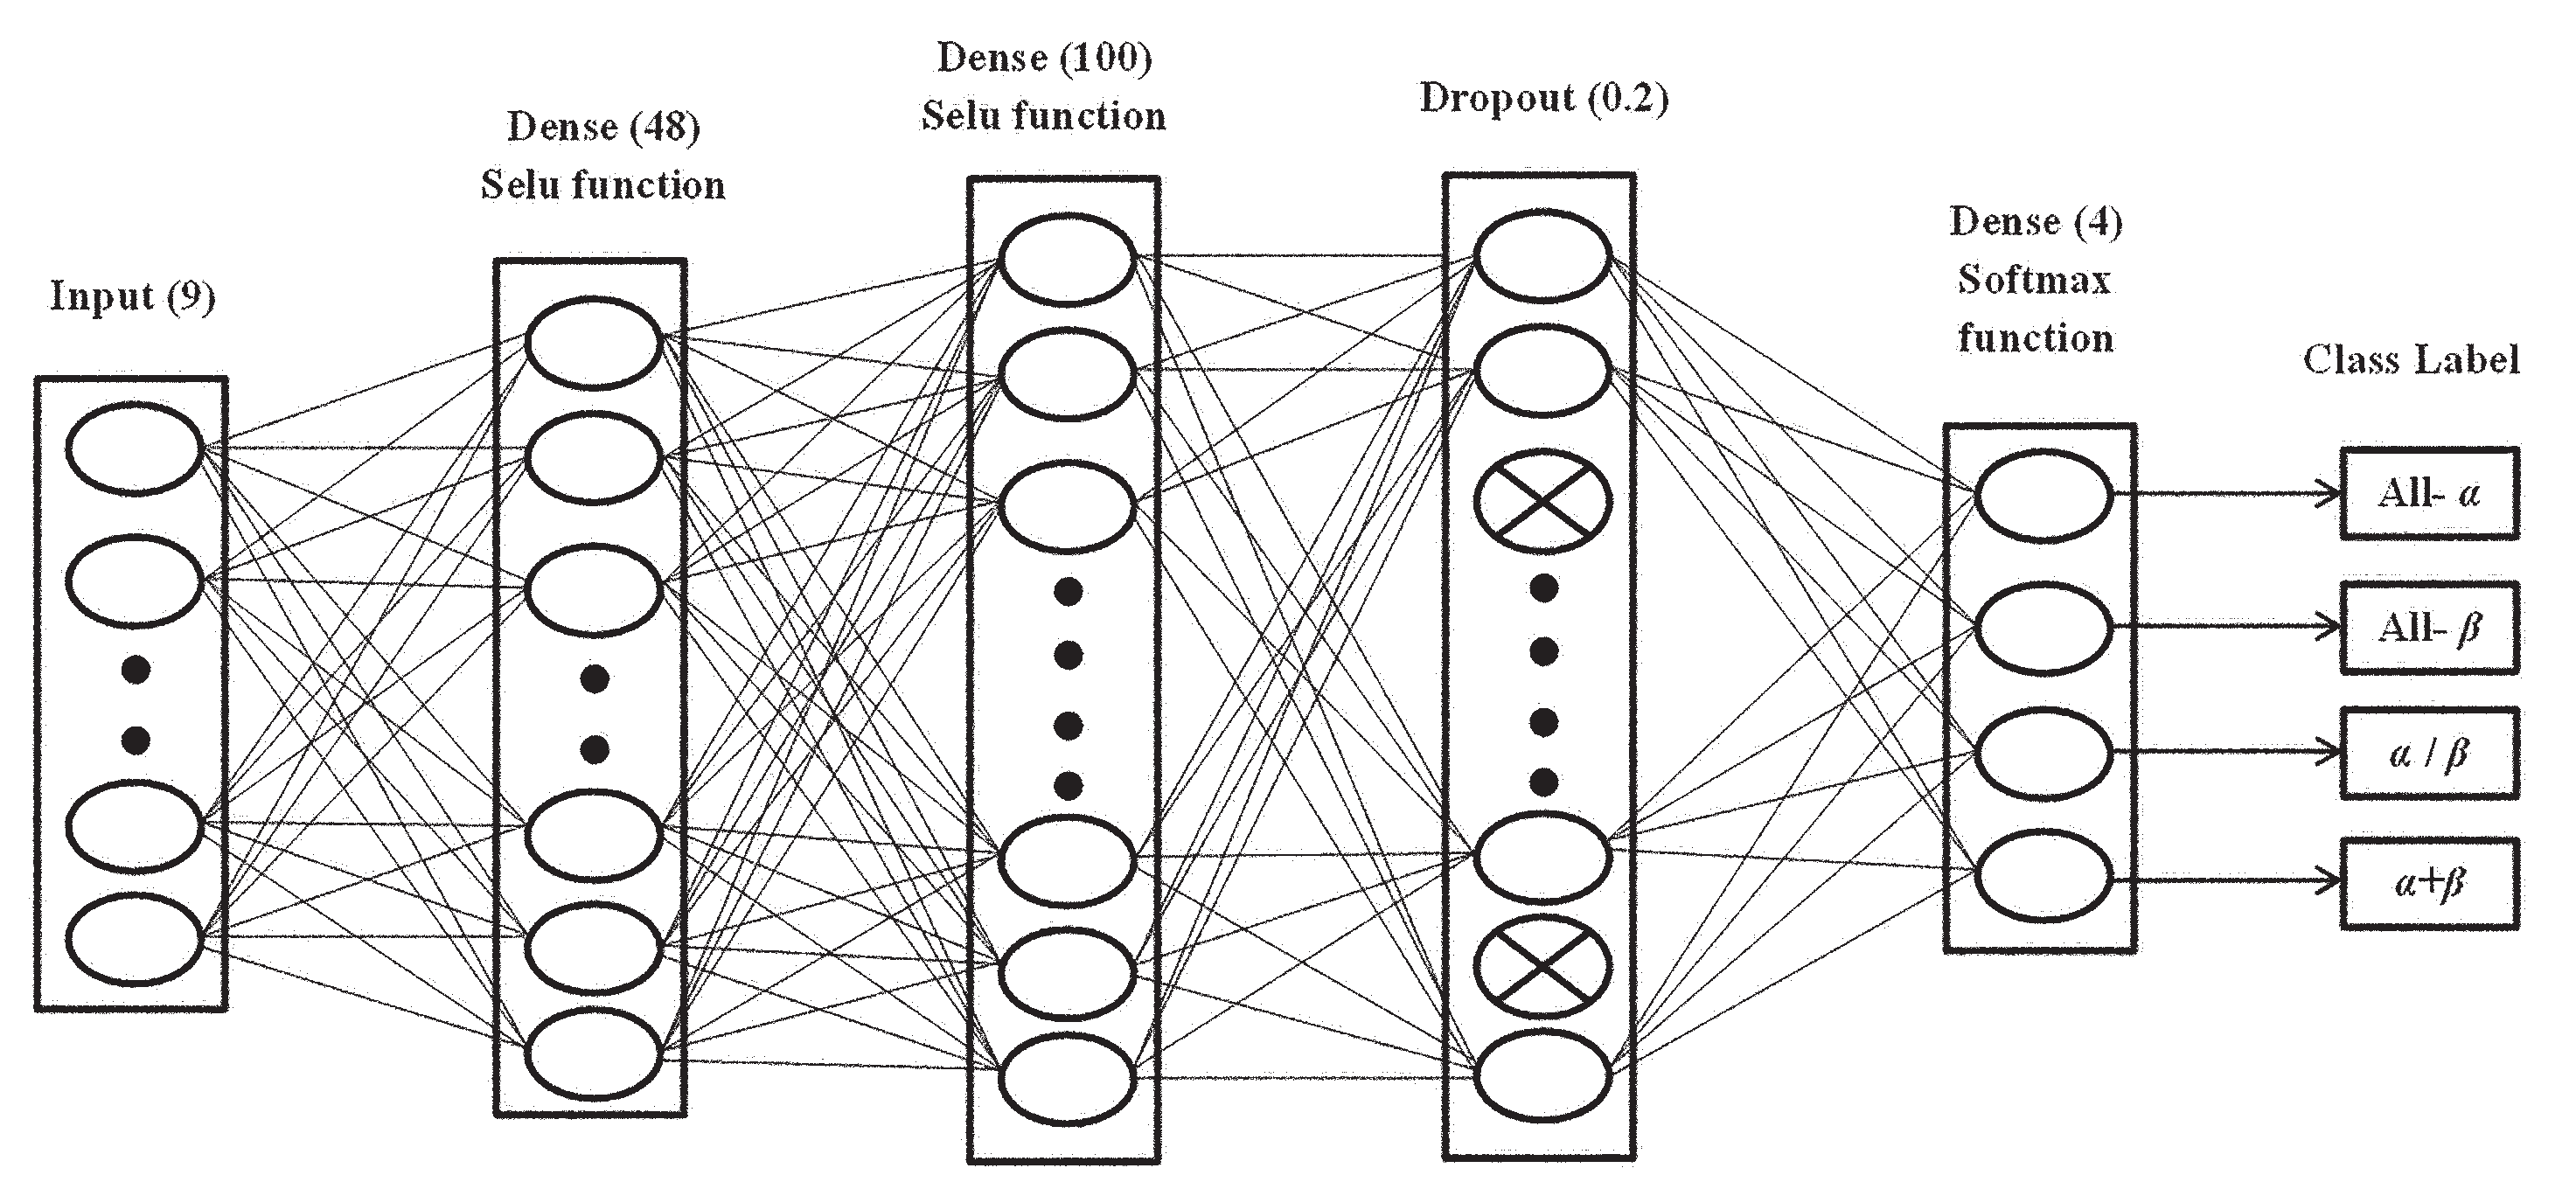
\includegraphics[width=320pt]{fig2.eps}
	% figure caption is below the figure
	\caption{A pruned neural network}
	\label{fig2}       % Give a unique label
\end{figure}

\subsection{Example of subsection 3}
When you prepare a reference list for your article, please use templates for bibliography formatting provided at the end of this document. You can find there templates and examples for formatting different possible categories of references such as periodicals, books, Chapters in books, Book series, Reports, Handbooks, Published Conference Proceedings, Theses (B.S., M.S.) and Dissertations (Ph.D.), Standards, On-Line Sources. Be sure that you provided all the information about the reference. It should be written correctly. Follow the format of the names and surnames of the authors of the sources. Pay attention that we use Western name order: initials (first name) should be before the respective surname (last name). The order and punctuation in reference formatting should be used properly according to the respective category template. Write in the commented line before each command \texttt{$\backslash$bibitem\{...\}} the name of the category of the respective source, e.g., \% Periodicals, \% Published Conference Proceedings, \% Chapters in books, etc.

Also, if you prefer, you can use the BibTeX system to manage your bibliography. In such a case you should take IEEE style (use IEEEtran.bst in your LaTeX files). All the necessary information, templates, and style files are provided on the page with Instructions for Authors at the CSJM site (https://www.math.md/publications/csjm/instructions-authors/).

The main recommendation concerns the requirement to provide more detailed information about references if possible, including page numbers, DOI, ISSN, ISBN, etc.

\textbf{Note.} The number of example references in the bibliography list in this template is rather wide to help the authors to orientate. However, the authors should provide in their article the required number of references, but not too many. The numbering of sources in the bibliography should correspond to the order of their appearance in the article. 

\section{Title of section 4}\label{sect4}
Below there are examples of the Definition, Theorem, Corollary, and Algorithm layout followed by some pieces of the text of the published articles. Also, patterns for Example and Table are given. These layouts are recommended, but not obligatory.

Tables must have caption located above the table (see Table \ref{tab1}).

\subsection{Example of subsection 1}\label{subsect1}
\textbf{Definition 1 \cite{1}.} \textit{$u_1, u_2, \ldots, u_n$ are the $N$ inlets to the permutation networks.} 

\begin{theorem}\cite{3}
	The number of mistakes made by the on-line perceptron algorithm, on a set $A$ that has a solution to the problem, is at most $(2R/\gamma)^2$, where $R=\max\|a_i\|$ and $\gamma$ is the size of the margin.
\end{theorem}

...

Diagnosis is defined as a process of exact failure cause
localization. Once the failure is detected, it is the
responsibility of the maintenance engineer to recognize the
effects, to analyze information, to interpret the various error
messages and indications, and to leave with the true diagnosis of
the situation in term of components having caused the failure and
the reason of their failures. When the diagnosis is completed, the
replacement or the repair of the component at the origin of the
failure is the following defect correction stage. The companies
are thus confronted with this double economic challenge:
\begin{itemize}
	\item to increase the productivity by increasing availability of
	their equipments production;
	
	\item to reduce the maintenance costs.
\end{itemize}

\subsection{Example of subsection 2}\label{subsect2}

\textbf{Corollary 1} \textit{For a graph $K_n$ with $n\ge 3$, we have:}
\[
\left\{ {{\begin{array}{*{20}c}
		{\overline \chi (K_n )=\frac{9k^2-7k}{3}\quad \mbox{if}\quad n=3k} \quad\quad\quad\\
		{\overline \chi (K_n )=\frac{9k^2+k-2}{2}\quad \mbox{if}\quad n=3k+1} \ \  \\
		{\overline \chi (K_n )=\frac{9k^2+5k-2}{2}\quad \mbox{if}\quad n=3k+2} \\
		\end{array} }} \right. .
\]

\noindent \textbf{Corollary 2} \textit{For a graph}
\textbf{K}$_n$ \textit{with} $n\ge3$, \textit{we have}:

$$
\left\{
\begin{array}{l}
\overline{\chi}(\textbf{K}_n)=\frac{9k^2-7k}{3} \hspace{1.0cm} \text{if} \hspace{0.5cm} n=3k\\
\overline{\chi}(\textbf{K}_n)=\frac{9k^2+k-2}{2} \hspace{0.8cm} \text{if} \hspace{0.5cm} n=3k+1\\
\overline{\chi}(\textbf{K}_n)=\frac{9k^2+5k-2}{2} \hspace{0.65cm} \text{if} \hspace{0.5cm} n=3k+2\\
\end{array}
\right.
$$

\subsubsection{Example of Subsubsection 1}\label{subsubsect1}

\textbf{Example 1} \textit{Let $A=Q[x^{2}, xy] \subseteq  Q[x, y]$ and use the degree lexicographical order with $x>y$. The set $F=\{x^{2}, xy\}$ is a SAGBI basis for $A$. Let $g=x^{3}y+x^{2}$ and $h=x^{4}+x^{2}y^{2}$ in $A$. A Hilbert basis for the set of solutions of the equation (3) is:} 
\[
{\begin{array}{*{20}c}
	{\vec {v}_1 =(0,0,1,0,1,0),} \hfill & {\vec {v}_2 =(0,1,0,1,0,0),} \hfill & 
	{\vec {v}_3 =(0,2,0,0,0,1),} \hfill \\
	{\vec {v}_4 =(1,0,0,1,1,0),} \hfill & {\vec {v}_5 =(1,1,0,0,1,1),} \hfill & 
	{\vec {v}_6 =(2,0,0,0,2,1).} \hfill \\
	\end{array} }
\]



\begin{table}[htbp]
	\caption{Distances between image feature vectors} \vspace{3mm}
	\begin{tabular}
		{|p{34pt}|p{44pt}|p{44pt}|p{44pt}|p{44pt}|p{44pt}|} \hline &
		$V(I_{1} )$& $V(I_{2} )$& $V(I_{3} )$& $V(I_{4} )$&
		$V(I_{5} )$ \\
		\hline $V(I_{1} )$& 0& 571.3183& 293.0381& 675.6527&
		319.3169 \\
		\hline $V(I_{2} )$& 571.3183& 0& 599.5098& 359.3718&
		618.9163 \\
		\hline $V(I_{5} )$& 319.3169& 618.9163& 361.6215& 712.8829&
		0 \\
		\hline
	\end{tabular}
	\label{tab1}
\end{table}

\subsection{Example of subsection 3}
In case of d-convex graph here we have always equality
$|D|=n+m+2$. Let us denote by $\Gamma(x)$ the neighborhood of
vertex $x$, i.e. $\Gamma(x) = \{ y\in X | x\sim y \} $.

\begin{definition}
\bf{[5].} \it{A vertex $y$ is called copy for vertex $x\: (x \neq
y)$, in graph $G=(X;\: U)$ if $\Gamma(x) = \Gamma(y)$.}
\end{definition}

Let $T$ be a tree with at least 3 vertexes and $T_0$ a sub-graph
of $T$, that consists of all vertexes and edges of $T$, without
those suspended. So, for each unsuspended vertex $x$ from $T$, we
have a uniquely correspondent vertex $\bar x$ from $T_0$, and for
each vertex of $T_0$ we have a uniquely correspondent vertex from
$T$. Let $L(T,\: T_0)$ be a graph obtained from $T$, $T_0$ and by
adding the following edges: every vertex $\bar x$ of $T_0$ will be
adjacent with all vertexes from $\Gamma(x)$ from $T$, where $x$
and $\bar x$ are correspondent vertexes. It is easy to see that in
graph $L(T,\: T_0)$ every vertex of degree at least 3 has a unique
copy and there are no suspended vertexes.

The next theorem is true:

\begin{theorem}
\bf{[6].} \it{If $T$ is a tree with at least 3 vertexes, then
graph $G = L(T,\: T_0)$ is d-convex simple and planar.}
\end{theorem}

...

Let $\V$ be a finite generating set of the monoid of nonnegative
integer solutions
$(\psi_0,\psi_1,\ldots,\psi_m,\eta_1,\ldots,\eta_m,\eta_0)$ of:
\begin{equation}\label{miller4.1}
\psi_0 \mdeg(g) + \sum_{\nu=1}^m \psi_{\nu} \mdeg(f_{\nu}) =
\sum_{\nu=1}^m \eta_{\nu} \mdeg(f_{\nu}) + \eta_0 \mdeg(h).
\end{equation}

...

\begin{algorithm}\label{millerAlg2ref} \hspace{1cm} \\
\framebox[1.1\width]{
\begin{minipage}[c]{.8\textwidth}
Input: $g,h \in A$, a finite SAGBI basis $F$ for $A$\\
Output: A syzygy family $\mathrm{SyzFam}(g,h)$ for $g$ and $h$\\
Initialisation: $\mathrm{SyzFam}(g,h):=\emptyset$,
$\mathcal{PV}:=\emptyset$\\
Compute a generating set $\V$ for the solutions of
system~(\ref{miller4.1}).\\
$\mathcal{PV}:=\{\vec{v} \in \V : c_0 = d_0 = 1\}$\\
For Each $\vec{v} \in \mathcal{PV}$:\\
\makebox{$\hspace{1.5em}$} $s_{\vec{v}}:=\lc(H^{\vec{v}^r})\cdot
G^{\vec{v}^l} -
\lc(G^{\vec{v}^l})\cdot H^{\vec{v}^r}$\\
$ \mathrm{SyzFam}(g,h):=\bigcup_{\vec{v}\in \mathcal{PV}}
\{s_{\vec{v}}\} $
\end{minipage}
}
\end{algorithm}

An implementation of this algorithm is included in the author's
Maple package for SAGBI and SAGBI-Gr\"obner computations,
see~\cite{myMaplePackage}. For calculating the Hilbert bases the
Maple package uses Dmitrii~V. Pasechnik's implementation of the
algorithm described in~\cite{PasechnikHB}.

As an application of Algorithm~\ref{millerAlg2ref} we consider
examples 4.7 and 5.2 in~\cite{millerSG}.
\begin{example}
Let $A = \mathbb{Q}[x^2,xy] \subseteq \mathbb{Q}[x,y]$ and use the
degree lexicographical order with $x > y$. The set $F=\{x^2,xy\}$
is a SAGBI basis for $A$. Let $g = x^3 y + x^2$ and $h = x^4 + x^2
y^2$ in $A$. A Hilbert basis for the set of solutions of the
equation~(\ref{miller4.1}) is:
\[ \begin{array}{ccc}
\vec{v_1} = (0,0,1,0,1,0), & \vec{v_2} = (0,1,0,1,0,0), &
\vec{v_3} =
(0,2,0,0,0,1), \\
\vec{v_4} = (1,0,0,1,1,0), & \vec{v_5} = (1,1,0,0,1,1), &
\vec{v_6} = (2,0,0,0,2,1).
\end{array}\]
Thus $\mathcal{PV} =\{\vec{v_5}\}$, so by
Algorithm~\ref{millerAlg2ref} a syzygy family for $(g,h)$ is
$\{G^{(1,1,0)} - H^{(0,1,1)}\} =\{ -x^3 y^3 + x^4\}$.

In the original version of this example (example~4.7 in
\cite{millerSG}) the syzygy family was $\{-x^5 y^3 + x^6, -x^3 y^3
+ x^4 \}$ instead. It should however be noted (as proved in
example~5.2, \cite{millerSG}) that the extra syzygy polynomial
$-x^5 y^3 + x^6$ SI-reduces to zero over $\{g,h\}$. Thus this
extra polynomial does not affect the final result of
SAGBI-Gr\"obner basis computations.
\end{example}

\section{Conclusion}\label{sect5}
In this paper, the instructions for preparing an article for 
publishing in Computer Science Journal of Moldova are given.

Articles prepared in Word or using the styles other than csjmol.sty for formatting are not taken into consideration by CSJM Editorial Board.

We consider only the articles with a good level of English and prepared using this template and CSJM style. 

\textbf{Acknowledgments.} {\ldots} has supported part of the research for this paper.



%%% You can use BibTeX system to manage your bibliography. In such case you should take IEEE style (use IEEEtran.bst in your LaTeX files).

%\bibliographystyle{IEEEtran}     % Sets the bibliography style "IEEEtran.bst" to
                                                             % be used in this document.
%\bibliography{references}            % Use this command for including your 
                                                              % bibliography written in file "references.bib"
                                                              % created with BibTeX 



% Standard bibliography commands in LATEX
\begin{thebibliography}{99}%\itemsep-.3em
% ***\textbf{Periodicals}
% \textit{Basic Format:	}
%(Ed.CSJM): 

% Periodicals
\bibitem{1} \textcolor{red}{
	J. K. Author, ``Name of paper,'' \textit{Title of Periodical}, vol. x, no. x, pp. xxx--xxx, Abbrev. Month, year. 
	}

%or

% Periodicals
\bibitem{2} \textcolor{red}{
J. K. Author, ``Name of paper,'' \textit{Abbrev. Title of Periodical}, vol. x, no. x, pp. xxx--xxx, Abbrev. Month, year. 
}

%\textit{Examples: }

% Periodicals
\bibitem{3} M. Ito \textit{et al}., ``Application of amorphous oxide TFT to electrophoretic display,'' \textit{J. Non-Cryst. Solids}, vol. 354, no. 19, pp. 2777--2782, Feb. 2008. 

% Periodicals
\bibitem{4} R. Fardel, M. Nagel, F. Nuesch, T. Lippert, and A. Wokaun, ``Fabrication of organic light emitting diode pixels by laser-assisted forward transfer,'' \textit{Appl. Phys. Lett.}, vol. 91, no. 6, Aug. 2007, Art.ID. 061103. 

% Periodicals
\bibitem{5} J. Zhang and N. Tansu, ``Optical gain and laser characteristics of InGaN quantum wells on ternary InGaN substrates,'' \textit{IEEE Photon. J}., vol. 5, no. 2, Apr. 2013, Art no. 2600111. 

% Periodicals
\bibitem{6} J. U. Buncombe, ``Infrared navigation---Part I: Theory,'' \textit{IEEE Trans. Aerosp. Electron. Syst.}, vol. AES-4, 
no. 3, pp. 352--377, Sep. 1944.

% Periodicals
\bibitem{7} S. Azodolmolky \textit{et al}., Experimental demonstration of an impairment aware network planning and operation tool for transparent/translucent optical networks,'' \textit{J. Lightw. Technol.}, vol. 29, no. 4, pp. 439--448, Sep. 2011. 

% Periodicals
\bibitem{8} H. Eriksson and P. E. Danielsson, ``Two problems on Boolean memories,'' \textit{IEEE Trans. Electron. Devices}, vol. ED-11, no. 1, pp. 32--33, Jan. 1959. 

% Periodicals
\bibitem{9} F. Aronowitz, ``Theory of traveling-wave optical maser,'' \textit{Phys. Rev.}, vol. 134, pp. A635--A646, Dec. 8, 1965. 

% Periodicals
\bibitem{10} Ye. V. Lavrova, ``Geographic distribution of ionospheric disturbances in the F2 layer,'' \textit{Tr. IZMIRAN}, vol. 19, no. 29, pp. 31--43, 1961 (Transl.: E. R. Hope, Directorate of Scientific Information Services, Defence Research Board of Canada, Rep. T384R, Apr. 1963). 

% Periodicals
\bibitem{11}  E. P. Wigner, ``On a modification of the Rayleigh--Schrodinger 
perturbation theory,'' \textit{Math. Naturwiss. Anz. Ungar. Akad. Wiss.}, vol. 53, p. 475, 1935. (in German)

% Periodicals
\bibitem{12}  E. H. Miller, ``A note on reflector arrays,'' \textit{IEEE Trans. Antennas Propag.}, to be published. 
%\textit{*** Always use this style when the paper has been accepted or scheduled for a future publication, i.e., do not use ``to appear in.''*** }

% Periodicals
\bibitem{13}  W. Rafferty, ``Ground antennas in NASA's deep space 
telecommunications,'' \textit{Proc. IEEE,} vol. 82, no. 5, pp. 636--640, May 1994. 

% Periodicals
\bibitem{14}  L. T. Wu \textit{et al.}, ``Real-time analytic sensitivity method for transient security assessment and prevent control,'' \textit{Proc. Inst. Elect. Eng., }vol. 135, pt. C, pp. 107--117, Mar. 1988. 
%\textit{***Authors may refer to this journal as Proc. IEE, but the abbreviation must be as listed above. Proc. IEE is printed in the U.K. and must not be confused with the Proc. IEEE.*** }

% Periodicals
\bibitem{15}  \textit{Special Issue on Artificial Neural Network Applications}, \textit{Proc. IEEE}, vol. 84, pp. 1353--1576, Oct. 1996. 

%\textbf{(Ed.CSJM): 

% Periodicals
\bibitem{PasechnikHB}
D.V. Pasechnik. ``On computing Hilbert bases via the Elliot-MacMahon algorithm,'' \textit{Theoretical Computer Science}, vol. 263, no. 1-2, pp.
37--46, 2001. 

%\textbf{(Ed.CSJM): examples with information in original language}

% Periodicals
\bibitem{17}  S. Cretu and A. Popescu, ``Semantic and pragmatic aspects of the meaning sentence,'' \textit{Meridian ingineresc}, no. 3, pp. 18--23, 2013. (in Romanian)
% ``Aspecte semantice si pragmatice ale sensului propozitiei in limbaj natural,'' \textit{Meridian ingineresc}).

% Periodicals
\bibitem{18}  B.A. Sevastyanov and V.P. Chistyakov, ``On the number of input 
sequences corresponding to the output sequences of a finite automaton,'' 
\textit{Review of Applied and Industrial Mathematics}, vol. 1, no. 1, pp. 96--107, 1994. (in Russian)
% "О числе входных последовательностей, соответствующих выходной последовательности конечного автомата,” \textit{Обозрение прикладной и промышленной математики}

%\textbf{(Ed.CSJM): examples with information about electronic sources 	included with the print reference }

% Periodicals
\bibitem{19} K. Kolikov, G. Krastev, Y. Epitropov and D. Hristozov, ``Analytically determining of the absolute inaccuracy (error) of indirectly measurable variable and dimensionless scale characterising the quality of the 
experiment,'' \textit{Chemometr Intell Lab}, vol. 102, pp. 15--19, 2010. Available: http://dx.doi.org/10.1016/j.chemolab.2010.03.001.

% Periodicals
\bibitem{20} K. Kolikov, G. Krastev, Y. Epitropov and A. Corlat, ``Analytically 
determining of the relative inaccuracy (error) of indirectly measurable 
variable and dimensionless scale characterising the quality of the 
experiment,'' \textit{Computer Science Journal of Moldova}, vol. 20, no. 1, pp. 
314--331, 2012. Available: 
http://www.math.md/en/publications/csjm/issues/v20-n1/11035/.

%***\textbf{Books and / Chapters in books/ Book series (Ed.CSJM):}

%\textit{Basic Format: }

%(Ed.CSJM): 

% Books
\bibitem{21} \textcolor{red}{
J. K. Author, \textit{Title of His Published Book}, x-th ed., vol. x, J. S. Editor, Ed. City of Publisher, (only U.S. State), Country: Abbrev. of Publisher, year, xxx p.
} 

%\textit{or}

% Chapters in books
\bibitem{22} \textcolor{red}{
J. K. Author, ``Title of chapter in the book,'' in \textit{Title of His Published Book} (Title of Series, vol./no. x), x-th ed., J. S. Editor\_1 and A. B. Editor\_2, Eds. City of Publisher, (only U.S. State), Country: Abbrev. of Publisher, year, ch. x, sec. x, pp. xxx--xxx. 
}
%\textit{Examples: }

% Books
\bibitem{23} B. Klaus and P. Horn, \textit{Robot Vision. }Cambridge, MA, USA: MIT Press, 1986, 480 p.  

% Chapters in books
\bibitem{24} L. Stein, ``Random patterns,'' in \textit{Computers and You, }J. S. Brake, Ed. New York, NY, USA: Wiley, 1994, pp. 55--70. 

% Chapters in books
\bibitem{25} R. L. Myer, ``Parametric oscillators and nonlinear materials,'' in 
\textit{Nonlinear Optics}, vol. 4, P. G. Harper and B. S. Wherret, Eds. San Francisco, CA, USA: Academic, 1977, pp. 47--160. 

% Books
\bibitem{26} M. Abramowitz and I. A. Stegun, Eds., \textit{Handbook of Mathematical Functions }(Applied Mathematics Series 55). 
Washington, DC, USA: NBS, 1964, pp. 32--33. 

% Chapters in books
\bibitem{27} E. F. Moore, ``Gedanken-experiments on sequential machines,'' in 
\textit{Automata Studies }(Ann. of Math. Studies, no. 1), C. E. Shannon and J. McCarthy, Eds. Princeton, NJ, USA: Princeton Univ. Press, 1965, pp. 129--153. 

% Books
\bibitem{28} Westinghouse Electric Corporation (Staff of Technology and Science, Aerospace Div.), \textit{Integrated Electronic Systems}. Englewood Cliffs, NJ, USA: Prentice-Hall, 1970. 

% Chapters in books
\bibitem{29} M. Gorkii, ``Optimal design,'' in \textit{Dokl. Akad. Nauk SSSR}, vol. 12, pp. 111--122, 1961 (Transl.: in L. Pontryagin, Ed., \textit{The Mathematical Theory of Optimal Processes. }New York, NY, USA: Interscience, 1962, ch. 2, sec. 3, pp. 127--135). 

% Chapters in books
\bibitem{30} A. Histace, ``Image restoration---Recent advances and applications,'' in \textit{Super-Resolution Restoration and Image Reconstruction for Passive Millimeter Wave Imaging. }Rijeka, Croatia: InTech, 2012, pp. 25--45. 

%\textbf{(Ed.CSJM):}

% Book series
\bibitem{31} M.A. Henning and A. Yeo, \textit{Total domination in graphs} (Springer Monographs in Mathematics), New York, NY, USA: Springer, 2013.

% Book series
\bibitem{32} M.C. Golumbic, \textit{Graph Theory and Perfect Graphs }(Annals of Discrete Mathematics, vol. 57), Amsterdam, North-Holland: North-Holland Publishing Co., 2004, 340 p. ISBN: 978-0-444-51530-8. 

% Chapters in books or Book series
\bibitem{33} R. Canetti, C. Dwork, M. Naor and R. Ostrovsky, ``Deniable 
Encryption,'' in \textit{Advances in Cryptology - CRYPTO 1997 }(Lecture Notes in Computer Science, vol. 1294), Berlin, Heidelberg, New York: Springer-Verlag Berlin Heidelberg, 1997, pp. 90--104.

% Chapters in books or Book series
\bibitem{34} R. Diaconescu, ``Three decades of institution theory,'' in \textit{Universal Logic: an Anthology} (Studies in Universal Logic), J.-Y. B\'{e}ziau, Ed. Birkh\"{a}user Basel, 2012, pp. 309--322. 

% Chapters in books or Book series
\bibitem{millerSG}
J. Lyn Miller. ``Effective algorithms for intrinsically computing {SAGBI}-{G}r\"obner bases in a polynomial ring over a field," in \textit{Gr\"obner bases and applications} (London Mathematical Society Lecture Note Series vol. 251), Cambridge: Cambridge University Press, 1998, pp. 421--433.

%\textbf{(Ed.CSJM): example of book with information in original language}

% Books
\bibitem{36} D. Hristozov, I. Mladenov, S. Armenski, N. Andreev, M. Minev, and H. Manev, \textit{Lab physics practicum}, Sofia, Bulgaria: Science and art, 1990. (in Bulgarian)
% \textit{Лабораторен практикум по физика}.

%\textbf{(Ed.CSJM): example of chapter in the book with information about editors}

% Chapters in books
\bibitem{37} P. Ekman, ``Basic Emotions'' in \textit{Handbook of Cognition and Emotion}, T. Dalgleish and M. Power, Eds. New York, NY, USA: John Wiley and Sons Ltd., 1999, pp. 45--60. 

%\textbf{(Ed.CSJM): example of chapter in book with information about 	electronic sources included with the print reference }

% Chapters in books
\bibitem{38} A. Belovs, A. Rosmanis and J. Smotrovs, ``Multi-letter Reversible and Quantum Finite Automata,'' in \textit{Developments in Language Theory }(Lecture Notes in Computer Science, vol. 4588), Springer Berlin Heidelberg, 2007, pp. 60-71. ISBN: 978-3-540-73207-5. 
Available: DOI: 10.1007/978-3-540-73208-2{\_}9.

%\textbf{\textit{Reports }}

%\textit{Basic Format: }

% Reports
\bibitem{39} \textcolor{red}{
J. K. Author, ``Title of report,'' Abbrev. Name of Co., City of Co., 
Abbrev. State, Country, Rep. xxx, year.
}
%\textit{Examples: }

% Reports
\bibitem{40} E. E. Reber, R. L. Michell, and C. J. Carter, ``Oxygen absorption in the earth's atmosphere,'' Aerospace Corp., Los Angeles, CA, USA, Tech. Rep. 
TR-0200 (4230-46)-3, Nov. 1988. 

% Reports
\bibitem{41} J. H. Davis and J. R. Cogdell, ``Calibration program for the 16-foot 
antenna,'' Elect. Eng. Res. Lab., Univ. Texas, Austin, Tech. Memo. 
NGL-006-69-3, Nov. 15, 1987. 

% Reports
\bibitem{42} R. E. Haskell and C. T. Case, ``Transient signal propagation in lossless isotropic plasmas,'' USAF Cambridge Res. Labs., Cambridge, MA, Rep. 
ARCRL-66-234 (II), 1994, vol. 2. 

% Reports
\bibitem{43} M. A. Brusberg and E. N. Clark, ``Installation, operation, and data 
evaluation of an oblique-incidence ionosphere sounder system,'' in ``Radio 
Propagation Characteristics of the Washington--Honolulu Path,'' Stanford 
Res. Inst., Stanford, CA, USA, Contract NOBSR-87615, Final Rep., Feb. 1995, 
vol. 1. 

% Reports
\bibitem{44} P. Diament, S. L. Richert, and W. L. Lupatkin, ``V-line surface-wave radiation and scanning,'' Dep. Elect. Eng., Columbia Univ., New York, Sci. Rep. 85, Aug. 1991. 

%\textbf{\textit{Handbooks }}

%\textit{Basic Format: }

% Handbooks
\bibitem{45} \textcolor{red}{
\textit{Name of Manual/Handbook}, x ed., Abbrev. Name of Co., City of Co., Abbrev. State, year, pp. xxx-xxx. 
}
%\textit{Examples: }

% Handbooks
\bibitem{46} \textit{Transmission Systems for Communications}, 3rd ed., Western Electric Co., Winston-Salem, NC, 1985, pp. 44--60. 

% Handbooks
\bibitem{47} \textit{Motorola Semiconductor Data Manual}, Motorola Semiconductor Products Inc., Phoenix, AZ, 1989. 

% Handbooks
\bibitem{48} \textit{RCA Receiving Tube Manual}, Radio Corp. of America, Electronic Components and Devices, Harrison, 
NJ, Tech. Ser. RC-23, 1992. 

%\textbf{\textit{Published Conference Proceedings }}

%\textit{Basic Format: }

% Published Conference Proceedings
\bibitem{49}  \textcolor{red}{
J. K. Author, ``Title of paper,'' in \textit{Abbreviated Name of Conf.}, (location of conference is optional), year, pp. xxx--xxx. 
}
%\textit{Examples: }

% Published Conference Proceedings
\bibitem{50}  G. R. Faulhaber, ``Design of service systems with priority 
reservation,'' in \textit{Conf. Rec. 1995 IEEE Int. Conf. Commun.}, pp. 3--8. %\textit{*** If the year is given in the conference title, it may be omitted from the end of the reference as shown here.*** }

% Published Conference Proceedings
\bibitem{51}  S. P. Bingulac, ``On the compatibility of adaptive controllers,'' in 
\textit{Proc. 4th Annu. Allerton Conf. Circuit and Systems Theory}, New York, 1994, pp. 8--16. 

% Published Conference Proceedings
\bibitem{52}  W. D. Doyle, ``Magnetization reversal in films with biaxial 
anisotropy,'' in \textit{1987 Proc. INTERMAG Conf.}, pp. 2.2-1--2.2-6. 

% Published Conference Proceedings
\bibitem{53}  C. T. Meadow and D. W. Waugh, ``Computer assisted interrogation,'' in \textit{1991 Fall Joint Computer Conf., Proc. AFIPS Conf.,} vol. 29. Washington, DC: Spartan, 1991, pp. 381--394. 
%\textit{*** There is an $<$emspace$>$ between ``vol. 29.'' and ``Washington.''*** }

% Published Conference Proceedings
\bibitem{54}  P. C. Parks, ``Lyapunov redesign of model reference adaptive control systems,'' in \textit{1993 Joint Automatic Control Conf., Preprints}, pp. 485--491. 

% Published Conference Proceedings
\bibitem{55}  T. S. Hsia, ``System identification,'' in \textit{IEDM Tech. Dig.}, 1993, vol. 2, no. 8, pp. 6--13. 

%\textbf{(Ed.CSJM): example of paper in Conference Proceedings with 	information about electronic sources included with the print reference }

% Published Conference Proceedings
\bibitem{56} K. Kolikov, G. Krastev, Y. Epitropov and D. Hristozov, ``Method for analytical representation of the maximum inaccuracies of indirectly 
measurable variable (survey),'' in \textit{Proc. Anniversary Int. Conf. "Research and Education in Mathematics, Informatics and their Applications" -- REMIA 2010}, pp. 159--166. Available: http://hdl.handle.net/10525/1449

%\textbf{\textit{Theses (B.S., M.S.) and Dissertations (Ph.D.) }}

%\textit{Basic Format: }

% Theses (B.S., M.S.) and Dissertations (Ph.D.)
\bibitem{57}  \textcolor{red}{
J. K. Author, ``Title of thesis,'' M.S. thesis, Abbrev. Dept., Abbrev. Univ., City of Univ., Abbrev. State, year. }

% Theses (B.S., M.S.) and Dissertations (Ph.D.)
\bibitem{58} \textcolor{red}{ 
J. K. Author, ``Title of dissertation,'' Ph.D. dissertation, Abbrev. 
Dept., Abbrev. Univ., City of Univ., Abbrev. State, year.}

%\textit{Examples: }

% Theses (B.S., M.S.) and Dissertations (Ph.D.)
\bibitem{59}  J. O. Williams, ``Narrow-band analyzer,'' Ph.D. dissertation, Dept. 
Elect. Eng., Harvard Univ., Cambridge, MA, 1993. 

% Theses (B.S., M.S.) and Dissertations (Ph.D.)
\bibitem{60}  N. Kawasaki, ``Parametric study of thermal and chemical nonequilibrium nozzle flow,'' M.S. thesis, Dept. Electron. Eng., Osaka Univ., Osaka, Japan, 1993. 

% Theses (B.S., M.S.) and Dissertations (Ph.D.)
\bibitem{61}  N. M. Amer, ``The effects of homogeneous magnetic fields on developments of tribolium confusum,'' Ph.D. dissertation, Radiation Lab., Univ. 
California, Berkeley, Tech. Rep. 16854, 1995. 
%\textit{*** The state abbreviation is omitted if the name of the university includes the state name, i.e., ``Univ. California, Berkeley.''*** }

% Theses (B.S., M.S.) and Dissertations (Ph.D.)
\bibitem{62}  C. Becle, These de doctoral d'etat, Univ. Grenoble, Grenoble, France, 1968. 

%\textbf{\textit{Standards }}

%\textit{Basic Format: }

% Standards
\bibitem{63}  \textcolor{red}{
\textit{Title of Standard}, Standard number, date. 
}
%\textit{Examples: }

% Standards
\bibitem{64}  \textit{IEEE Criteria for Class IE Electric Systems}, IEEE Standard 308, 1969. 

% Standards
\bibitem{65}  \textit{Letter Symbols for Quantities}, ANSI Standard Y10.5-1968. 

%\textbf{C. On-Line Sources }

%\textbf{\textit{Books, Monographs }}

%\textit{Online Basic Format: }

% On-Line Sources (Books, Monographs)
\bibitem{66}  \textcolor{red}{
J. K. Author, ``Title of chapter in the book,'' in \textit{Title of Published Book}, xth ed. City of Publisher, State, Country: Abbrev. of Publisher, year, ch. x, sec. x, pp. xxx--xxx. [Online]. Available: http://www.web.com 
}
%\textit{Examples: }

% On-Line Sources (Books, Monographs)
\bibitem{67}  G. O. Young, ``Synthetic structure of industrial plastics,'' in 
Plastics, vol. 3, Polymers of Hexadromicon, J. Peters, Ed., 2nd ed. New 
York, NY, USA: McGraw-Hill, 1964, pp. 15--64. [Online]. Available: 
http://www.bookref.com.

% On-Line Sources (Books, Monographs)
\bibitem{68}  \textit{The Founders' Constitution}, Philip B. Kurland and Ralph Lerner, eds., Chicago, IL, USA: Univ. Chicago Press, 1987. [Online]. Available: 
http://press-pubs.uchicago.edu/founders/ 

% On-Line Sources (Books, Monographs)
\bibitem{69}  The Terahertz Wave eBook. ZOmega Terahertz Corp., 2014. [Online]. Available: 
http://dl.z-thz.com/eBook/zomega{\_}ebook{\_}pdf{\_}1206{\_}sr.pdf. Accessed on: May 19, 2014. 

% On-Line Sources (Books, Monographs)
\bibitem{70}  Philip B. Kurland and Ralph Lerner, eds., \textit{The Founders' Constitution. }Chicago, IL, USA: Univ. of Chicago Press, 1987, http://press-pubs.uchicago.edu/founders/. Accessed on: Feb. 28, 2010. 

%\textbf{\textit{Periodicals }}

%\textit{Basic Format: }

% On-Line Sources (Periodicals)
\bibitem{71}  \textcolor{red}{
J. K. Author, ``Name of paper,'' \textit{Abbrev. Title of Periodical}, vol. x, no. x, pp. xxx-xxx, Abbrev. Month, year. [Online]. Available: site/path/file. Accessed on: Month, Day, Year. 
}
%\textit{Examples: }

% On-Line Sources (Periodicals)
\bibitem{72}  J. S. Turner, ``New directions in communications,'' \textit{IEEE J. Sel. Areas Commun}., vol. 13, no. 1, pp. 11--23, Jan. 1995. 

% On-Line Sources (Periodicals)
\bibitem{73}  W. P. Risk, G. S. Kino, and H. J. Shaw, ``Fiber-optic frequency shifter using a surface acoustic wave incident at an oblique angle,'' \textit{Opt. Lett.}, vol. 11, no. 2, pp. 115--117, Feb. 1986. [Online]. Available: 
http://ol.osa.org/abstract.cfm?URI=ol-11-2-115 

%\textbf{\textit{Papers Presented at Conferences }}

%\textit{Basic Format: }

% On-Line Sources (Papers Presented at Conferences)
\bibitem{74} \textcolor{red}{
 J. K. Author. Title. presented at abbrev. Conference title. [Type of 
Medium]. Available: site/path/file 
}
%\textit{Example: }

% On-Line Sources (Papers Presented at Conferences)
\bibitem{75} Process Software Corp., MA. Intranets: Internet technologies deployed behind the firewall for corporate productivity. presented at INET'96 Annu. Meeting [Online]. Available: http://www.process.com/Intranets/wp2.htp 

%\textbf{\textit{Reports and Handbooks }}

%\textit{Basic Online Format: }

% On-Line Sources (Reports and Handbooks)
\bibitem{76} \textcolor{red}{
J. K. Author, ``Title of report,'' Abbrev. Name of Co., City of Co., 
Abbrev. State, Country, Rep. no., vol./issue, year. [Online]. Available: 
site/path/file 
}
%\textit{Basic Format: }

% On-Line Sources (Reports and Handbooks)
\bibitem{77} \textcolor{red}{
J. K. Author. (year, month). Title. Company. City, State, Country. [Type of Medium]. Available: site/path/file 
}
%\textit{Examples: }

% On-Line Sources (Reports and Handbooks)
\bibitem{78} R. J. Hijmans and J. van Etten, ``Raster: Geographic analysis and 
modeling with raster data,'' R Package Version 2.0-12, Jan. 12, 2012. 
[Online]. Available: \underline {http://CRAN.R-project.org/package=raster }

% On-Line Sources (Reports and Handbooks)
\bibitem{79} Teralyzer. Lytera UG, Kirchhain, Germany [Online]. Available: 
http://www.lytera.de/Terahertz{\_}THz{\_}Spectroscopy.php?id=home, Accessed on: Jun. 5, 2014. 

% On-Line Sources (Reports and Handbooks)
\bibitem{80} Linear Technology, Standalone linear Li-ion battery charger and dual synchronous buck converter,'' Rep. no. LTC3552, Datasheet., 2012. Accessed on Sep. 12, 2014. 

% On-Line Sources (Reports and Handbooks)
\bibitem{81} Bureau of Meteorology, "Bureau of Meteorology: Measuring Rainfall in Australia," 2009. [Online]. Available: http://www.bom.gov.au/climate/cdo/about/definitionsrain.shtml\\
{\#}meanrainfall. 

% On-Line Sources (Reports and Handbooks)
\bibitem{82} GeoBasisNRW, Cologne, Germany, ``ATKIS---Digitale Topographische Karte 
1:25.000 (DTK25),'' Bezirksregierung Koln, 2012. [Online]. Available: 
http://www.bezreg-koeln.nrw.de\\
/brkinternet/presse/publikationen/geobasis\\
/faltblattgeobasisatkis01.pdf 

% On-Line Sources (Reports and Handbooks)
\bibitem{83} K. Kagaku. Multipurpose chest phantom: Lungman. [Online]. Available: 
http://www.kyotokagaku.com/products/detail03\\/pdf/ph-1{\_}catalog.pdf. Accessed Apr. 17, 2014. 

% On-Line Sources (Reports and Handbooks)
\bibitem{84} Apple Inc., Palo Alto, CA, USA, ``Apple iPhone,'' Available: 
http://apple.com/iphone/. Accessed: Feb. 26, 2013.

%\textbf{\textit{Government Documents }}

%\textit{Basic Format: }

% On-Line Sources (Government Documents)
\bibitem{85}  \textcolor{red}{
Legislative body. Number of Congress, Session. (year, month day). 
\textit{Number of bill or resolution}, \textit{Title}. [Type of medium]. Available: site/path/file 
}
%\textit{Example: }

% On-Line Sources (Government Documents)
\bibitem{86}  U.S. House. 102nd Congress, 1st Session. (1991, Jan. 11). \textit{H. Con. Res. 1, Sense of the Congress on Approval of Military Action}. [Online]. Available: LEXIS Library: GENFED File: BILLS 

%\textbf{\textit{Patents }}

%\textit{Basic Format: }

% On-Line Sources (Patents)
\bibitem{87}  \textcolor{red}{
Name of the invention, by inventor's name. (year, month day). \textit{Patent Number }[Type of medium]. Available: site/path/file 
}
%\textit{Example: }

% On-Line Sources (Patents)
\bibitem{88}  Musical toothbrush with adjustable neck and mirror, by L.M.R. Brooks. (1992, May 19). \textit{Patent D 326 189 }[Online]. Available: NEXIS Library: LEXPAT File: DESIGN 

%\textbf{\textit{Manuals/Software }}

% On-Line Sources (Manuals/Software)
\bibitem{89} \textcolor{red}{
 L. Breimann. (2003). \textit{Manual on Setting Up, Using, and Understanding Random Forests v4.0. }[Online]. Available: 
http://oz.berkeley.edu/users/breiman/Using{\_}random{\_}forests\\
{\_}v4.0.pdf, Accessed on: Apr. 16, 2014. 
}

% On-Line Sources (Manuals/Software)
\bibitem{90}  M. Kuhn. \textit{The Caret Package. }(2012) [Online]. Available: 
http://cranr-project.org/web/packages/caret/caret.pdf 

% On-Line Sources (Manuals/Software)
\bibitem{91}  Antcom, Torrance, CA, USA. \textit{Antenna Products. }(2011) [Online]. Available: 
http://www.antcom.com /documents/catalogs /L1L2GPSAntennas.pdf, Accessed on: Feb. 12, 2014. 

% On-Line Sources (Manuals/Software)
\bibitem{myMaplePackage}
H. {\"O}fverbeck. \textit{HilbertSagbiSg, Maple packages for Hilbert,
	SAGBI and SAGBI-Gr{\"o}bner basis calculations.} (2005) [Online]. Available: 
http://www.maths.lth.se/matematiklu/personal/hans/maple

\end{thebibliography}


\vspace{2mm}
\begin{center}
\begin{parbox}{118mm}{\footnotesize
First\_name1 Last\_name1,    \hfill Received MMM DD, YYYY

First\_name2 Last\_name2, First\_name3 Last\_name3

\vspace{3mm}

First\_name1 Last\_name1

ORCID: \texttt{https://orcid.org/XXXX-XXXX-XXXX-XXXX}

Institution

Address

E--mail: \texttt{e-mail\_address1}

\vspace{2mm}

First\_name2 Last\_name2

ORCID: \texttt{https://orcid.org/XXXX-XXXX-XXXX-XXXX}

Institution

Address

E--mail: \texttt{e-mail\_address2}

\vspace{2mm}

First\_name3 Last\_name3

ORCID: \texttt{https://orcid.org/XXXX-XXXX-XXXX-XXXX}

Institution

Address

E--mail: \texttt{e-mail\_address3}

}

\end{parbox}
\end{center}

\end{document}
